%%% mode: latex
%%% TeX-master: t
%%% End:

\chapter{绪论}
\label{cha:intro}
% 学位论文文字排版的字号、行距、字距的大小,以版面清晰、容易辨识和阅读为原则。为统一起见,具体要求如下:
% \begin{enumerate}
%     \item 论文页眉,楷体,小二;
%     \item 章和节的题名用黑体,字号分别用三号和四号;
%     \item 正文内容用宋体,英文用Times New Roman,小四号;行间距1.5倍;正文注意两侧对齐。
% \end{enumerate}

% 绪论部分是整篇论文的导引,应包括选题背景、意义;国内外研究概况;前人研究中存在的问题或知识空白;进而引出本文的研究设想,简要给出全文各章节的主要内容、以及章节之间相互联系。

% 在写作中无论是研究背景及意义,还是国内外研究现状,要做到有依据都必须引用参考文献。通常情况下,绪论部分的参考文献应占全文参考文献的百分之80以上。参考文献的顺序必须是按照在文章中出现的先后顺序进行排列。

% 以下简要说明一下绪论部分的内容及各级标题格式等。

\section{Galerkin-Legendre离散化分数阶KGS方程组}

考虑分数阶KGS方程组的实数形式,现将其表示为四个独立方程:

\begin{align}
q_t &= \frac{1}{2}(-\Delta)^{\frac{\alpha}{2}}p - p\phi \label{eq:q} \\
p_t &= -\frac{1}{2}(-\Delta)^{\frac{\alpha}{2}}q + q\phi \label{eq:p} \\
\phi_t &= \psi \label{eq:phi} \\
\psi_t &= -(-\Delta)^{\frac{\beta}{2}}\phi - m\phi + |u|^2 \label{eq:psi}
\end{align}

其中$m=1$,且$|u|^2 = p^2 + q^2$。

\subsection{空间离散化}

选择Legendre多项式作为基函数,定义有限维近似空间:
\[ V_N = \text{span}\{P_k(x)\}_{k=0}^N \]
其中$P_k(x)$是Legendre多项式\cite{bloch2005ultracold,bloch2008many}
\begin{align}
V(x) = V_0 \sin^2(kx),
\end{align}
其中 $k = \pi / a$,$a$ 是晶格间距。$V_{0}$ 是光学晶格的深度,与激光束的强度成正比。这种周期性势能的存在与自由粒子相比显著改变了系统的性质。晶格深度通常以反冲能量 \(E_R = \hslash ^2k^2/2m\)的单位来表示,其中 \(m\) 是原子的质量。因此,三对在三个正交方向上反向传播的激光束将形成一个三维(3D)光学晶格,如图\ref{fig:optical_Bloch}(b)所示。
并且,可以使用光学势阱创建几乎任意形状的晶格。如图\ref{fig:optical_Bloch}(a) 增加一个驻波的激光强度,沿此方向的跃迁概率迅速减小到零\cite{jaksch1999entanglement},有效地创建了一个二维的晶格阵列。此外,对光学晶格参数的高度控制使得对超冷原子的使用非常灵活,其同样可以探索凝聚态物质系统中的各种情况。光晶格也可以用来实现冷原子在不同格点之间的隧穿,由此产生莫特绝缘相到超流相的相变和布洛赫振荡等现象\cite{HuiNingju2013}。目前,光晶格系统在模拟凝聚态系统方面已取得了非常显著的成果\cite{bloch2008many,petrov2004low,hadzibabic2006berezinskii,griffin1996bose,fallani2008bose,bouyer2009anderson,becker2010ultracold,clement2008density}。

\begin{figure}
\centering
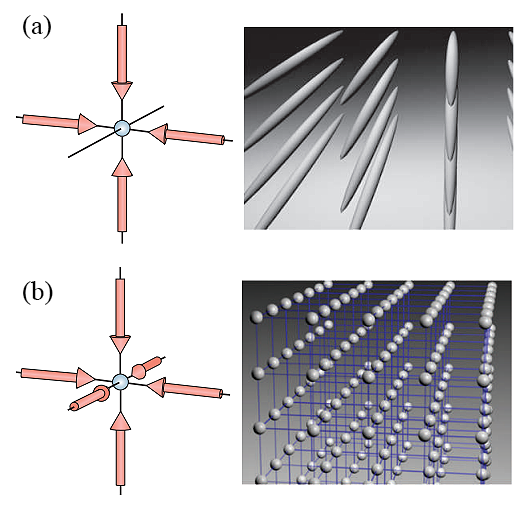
\includegraphics[width=8cm]{figures/chap01/optical_Bloch.png}
\vspace{-10pt}
\caption{由反向传播激光器创建的光晶格势的示意图:(a)准一维管的二维阵列和(b)三维简单立方晶格。图源自文献 \cite{bloch2005ultracold}。}\label{fig:optical_Bloch}
\end{figure}

%%%%%%%%%
%%%%%%%%%
\subsection{冷原子系统中的参数控制}

原子物理和量子光学提供了许多新方法来量子工程化光学晶格中的超冷原子。相对而言,在某些情况下原子物理学和量子光学不仅与凝聚态物理学相似,甚至在某些方面“超越”了凝聚态物理学。其中一个原因是冷原子在光学晶格中的实验提供了高度的控制。以下我们列出了一些可控制的参数。
\subsubsection{晶格几何和维度性}
通过设计激光束的方向、偏振、强度、相位和频率,几乎可以使用光学势实现任何晶格几何形状。此外,系统的维度也可以修改。研究人员已经使用反向传播的激光束创建了二维和三维的正方和立方晶格。例如,在三维系统中使用一维光学晶格,会生成一个二维系统的阵列。同样,在三维系统中使用二维光学晶格,会生成一个一维系统的阵列\cite{bloch2008many,petrov2004low,hadzibabic2006berezinskii,griffin1996bose}。
在每个子系统中,通过在这些维度中使用足够强的约束势,会使得所有相关能量都低于囚禁势的第一激发态\cite{griffin1996bose}。2010年,研究人员实现了混合维度的可能性\cite{lamporesi2010scattering}。相邻势阱之间的间距也可以修改—从 \(d = \lambda/2\)到 \(d = (\lambda/2) \sin(\theta/2)\),其中 \(\lambda\) 是形成晶格的反向传播光束的波长,改进之后可以使光束以某个角度 \(\theta\) 干涉。这种方法也可以用来解决单个晶格势阱。还有一种叠加的方法,即在现有晶格上添加不同频率的新晶格,也得到了很好的发展。这种方法允许创建双势阱晶格,即晶格的单位单元(周期性势阱结构中的一个最小重复单元)包含两个格点。它还允许通过叠加不同频的晶格或通过向晶格添加散斑辐射来创建准周期甚至随机系统\cite{fallani2008bose,bouyer2009anderson,clement2008density,dagnino2009vortex}。此外,更复杂的几何形状,如三角晶格,kagomé晶格等也可以实现\cite{becker2010ultracold,clement2008density}。同样的可以在环形光学晶格中实现周期性边界条件。

\begin{figure}
\centering
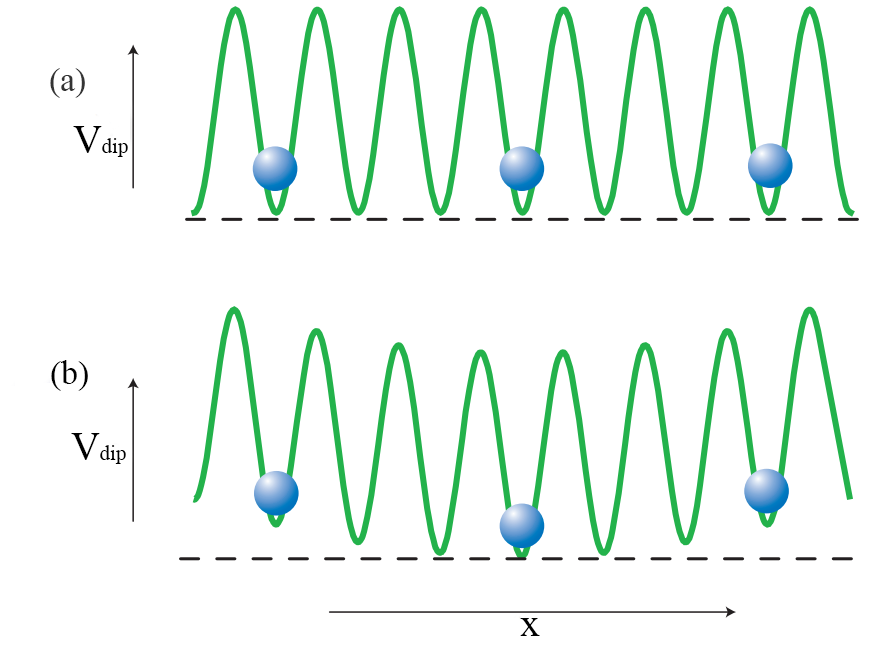
\includegraphics[width=8cm]{figures/chap01/lattice_potential.png}
\vspace{-10pt}
\caption{  光学晶格势。(a) 驻波干涉图样产生了一个周期性势,其中原子通过隧穿耦合在各个势阱之间移动。(b) 激光的高斯光束轮廓,一个残余的谐波捕获势,导致在周期性势上叠加了一个弱谐波限制。因此,整体捕获配置是不均匀的。图源自文献 \cite{bloch2005ultracold}。}
\label{fig:lattice_potential}
\end{figure}

\subsubsection{声子}
光学晶格是刚性且稳定的:它们不支持声子。但当晶格在光学腔中形成时,会出现一种有趣的情况:原子-光耦合可能足以改变腔共振。腔会影响原子,但原子会进行反作用,并可以产生类似声子的激发\cite{maschler2005cold},这导致超流相-莫特绝缘相(SF-MI)的转变 \cite{larson2008mott}。另一方面,声子在离子阱中起着显著作用,它们为离子-离子相互作用提供了主要机制\cite{mintert2001ion,porras2004effective}。

\subsubsection{隧穿和在位相互作用}

隧穿可以通过使用纯跃迁、激光辅助相干跃迁和晶格倾斜 (加速) 技术的组合在很大程度上进行控制\cite{Gao2023}。这种控制的显著例子是在晶格中创建人工磁场\cite{jaksch2003creation}。

尽管量子气体是非常稀薄的系统,密度通常在\( 10^{13} \) 到\( 10^{15} \)\( cm^{-3} \)
 之间,但它们的许多性质由粒子之间的相互作用支配。这些相互作用由散射长度表征,可以通过磁场中的费什巴赫共振 \cite{inouye1998observation,timmermans1999feshbach}或光学费什巴赫共振来修改,研究人员对此方法已做了理论解释\cite{fedichev1996influence}和实验验证\cite{thalhammer2005inducing}。在光学费什巴赫共振的原始提议中,激光非共振地耦合散射原子的基态与激发分子态。这种方法通常导致大的非弹性损失。后来,有科研团队提出了耦合共振分子能级与激发分子态\cite{bauer2009control}。通过这种方式实现了一种显著的无损失的新型控制。通过改变晶格势的形状,可以在偶极气体中将在位相互作用设置为零\cite{baranov2002ultracold}。

 \subsubsection{近邻和长程相互作用}
 通过计算莫特绝缘相中隧穿效应 \(t\) 获得的有效模型通常包含能量与\(t^2/U\)成比例的近邻相互作用,其中\(U\)表示在位相互作用。长程相互作用可以通过偶极力实现\cite{baranov2002ultracold,thalhammer2005inducing,lahaye2009physics}。科研人员通过凝聚玻色子-铬实现了超冷偶极气体的首次实验观察 \cite{griesmaier2005bose}。这里的偶极相互作用由铬原子的磁偶极介导;虽然这样的偶极相互作用很弱,但仍然能导致可观察到的效果\cite{stuhler2005magnetostriction}。通过处于基态的极性分子可以实现更强的电偶极-偶极相互作用 \cite{ni2008high}。在玻色-费米混合物中,玻色子可能介导费米子之间的相互作用,提供更强的相互作用。长程相互作用也可以在被捕获的离子系统中实现,并且通过平衡离子构型的声子振动介导。

  \subsubsection{自旋依赖的光学晶格和势能}
可以通过特定的配置创建依赖自旋的光学晶格,即两个具有线性偏振的反向传播激光束形成一定角度。利用这种类型的控制,具有不同内部超精细态 (自旋) 的原子可以经历不同的晶格势。因此,操纵自旋可以使原子向着相同或相反的方向移动\cite{jaksch1999entanglement,mandel2003controlled}。这种技术常用于调控原子间的相互作用。

除了光晶格势外,还可以对原子施加不同类型的外部势场。比如可以使用磁势,其形状目前可以在微米尺度上进行控制。此外,原子芯片可以产生具有更大梯度的磁势 \cite{della2007designing}。然而,最灵活的类型是光学势。光学势几乎可以呈现任意形状,并形成各种类型的光晶格:规则的、无序的、调制的等。特别是射频势能 \cite{hofferberth2006radiofrequency} 和全息掩模 \cite{bakr2009quantum}对原子势场的更加精确的操控提供了很大的可能性。

  

\subsection{周期性晶格中无相互作用的粒子:能带结构}

众所周知,无相互作用的单粒子在周期势中的能谱由具有带隙宽度的能带组成。因此,中性原子在周期势中由布洛赫波函数描述,就像固态晶体中的电子一样。在本节中,我们回顾了单粒子\cite{ashcroft1976solid}在一维周期势中的基本物理性质。进而推广到更高维度。

质量为$m$的粒子在周期势$V(x) = V(x + d)$中,周期为$d$,由薛定谔方程描述:
\begin{align}
\left[ \frac{p^2}{2m} + V(x) \right] \Phi_q^{(n)}(x) = E_q^{(n)} \Phi_q^{(n)}(x). \label{eq:1.6}
\end{align}
这个方程的解是布洛赫函数,根据布洛赫定理\cite{ashcroft1976solid},可以写成平面波和与势具有相同周期性的函数的乘积:
\begin{align}
\Phi_q^{(n)}(x) = e^{iqx} u_q^{(n)}(x), \label{eq:1.7}
\end{align}
其中:
\begin{align}
u_q^{(n)}(x + d) = u_q^{(n)}(x). \label{eq:1.8}
\end{align}
将方程(\ref{eq:1.7})引入方程(\ref{eq:1.6})得到$u_q^{(n)}(x)$的薛定谔方程:
\begin{align}
\left[ \frac{(p + \hslash {q})^2}{2m} + V(x) \right] u_q^{(n)}(x) = E_q^{(n)} u_q^{(n)}(x). \label{eq:1.9}
\end{align}
其中 \( q \) 由布洛赫定理引入,是准动量-周期势的平移对称性的量子数特征。
由于周期性,\( q \) 可以限制在第一布里渊区,即 \(-\pi/d < q < \pi/d\),其中 \( k_B = \pi/d \) 定义为布里渊区的动量。因为对于给定的 \( q \),薛定谔方程有许多解,因此布洛赫定理中出现索引 \( n \)(正整数)只是标记了能带。实际上,方程可以看作是一组本征值问题,每个 \( q \) 有一个,有无限多解。这些解具有离散的能谱,即著名的能带结构。注意,在无限周期势中,对于固定的 \( n \),\( E^{(n)}(q) \) 随 \( q \) 连续变化。第 \( n \) 个能带与第 \( (n+1) \) 能带之间有能隙隔开,该能隙取决于晶格结构和准动量。在低温极限下,粒子主要占据最低能带 \( n = 0 \),此时可以使用紧束缚近似来构造哈伯德模型。

值得注意的是,万尼尔函数是布洛赫函数在动量空间的傅里叶变换,它们形成一组完备的局域基\cite{abramowitz1964handbook}。而在深势阱极限下,万尼尔函数主要局限于单个格点附近,相对于布洛赫函数扩展到整个晶格,其更适用于紧束缚近似。此时万尼尔函数的基底可以用于构造哈伯德模型。换而言之,万尼尔函数是布洛赫函数的局域化表述,其具有以下形式:
\begin{align}
w_n(x - x_i) = \frac{1}{\sqrt{M}} \sum_q e^{-iqx_i} \Phi_q^{(n)}(x). \label{eq:3.15}
\end{align}

\subsubsection{哈伯德模型}

考虑光学晶格中的相互作用的玻色子和费米子,并推导出著名的哈伯德模型\cite{zhai2021ultracold}的哈密顿量。通过将场算符展开为最大局域的万尼尔波函数基矢,动能和相互作用模型都可以采取最简单的形式。首先考虑三维立方晶格中的相互作用的玻色子,$\hat{\psi}(\mathbf{r})$是玻色子的场算符,展开为
\begin{align}
\hat{\psi}(\mathbf{r}) = \sum_{m, \mathbf{R}_i} \hat{b}_{m,i} w_m(\mathbf{r} - \mathbf{R}_i),
\end{align}
其中$\hat{b}_{m,i}$是具有格点位置索引$i$和能带索引$m$的玻色子的湮灭算符。晶格模型的最一般形式为
\begin{align}
\hat{H} = - \sum_{ij} J_{ij}^{mm'} \hat{b}_{m,i}^\dagger \hat{b}_{m,j} + \frac{1}{2} \sum_{ijkl}^{mm'n'n'} \sum_{ij'j'} \hat{b}_{m_i}^\dagger \hat{b}_{m',j'}^\dagger \hat{b}_{n_i} \hat{b}_{n',j} - \mu \sum_{i,m} \hat{b}_{m,i}^\dagger \hat{b}_{m,i},
\end{align}
其中
\begin{align}
J_{ij}^{m} = - \int d^3 \mathbf{r} w_m(\mathbf{r} - \mathbf{R}_i) \left( - \frac{\hslash^2 {\nabla}^2}{2m} + V_{\text{lat}}(\mathbf{r}) \right) w_m(\mathbf{r} - \mathbf{R}_j),
\end{align}
和
\begin{align}
U_{ijkl}^{mm'n'n'} = \frac{4 \pi \hslash{k}^2 ds}{m} \int d^3 \mathbf{r} w_m(\mathbf{r} - \mathbf{R}_i) w_n(\mathbf{r} - \mathbf{R}_j) w_{m'}(\mathbf{r} - \mathbf{R}_k) w_{n'}(\mathbf{r} - \mathbf{R}_l).
\end{align}
相互作用能量约为 \(\sim \hslash a_s / (m a_{\text{har}}^3)\),其中 \(a_{\text{har}}\) 表示万尼尔波函数的典型宽度:\(a_{\text{har}} = 1 / (k_0 a^{1/4})\)。对于势深 \(V = a E_R\),带隙是 \(O(\hslash k^2 / (m a_{\text{har}}^2))\) 的量级。这里只关注于相互作用势远离散射共振的情况,即 \(k_F a_s \ll 1\),其中:\(k_F\) 为 \((6\pi^2 n)^{1/3}\)。对于典型的超冷原子气体密度,\(k_F \sim k_0\)。在超冷情况下,温度也可以远小于带隙,并且可以安全地忽略高能带中的能量分布。由于这两个原因,我们只能保留最低带 \(n = 0\)(即上节中提到的低温极限下)。在此之后我们将忽略带索引。由于最低带的万尼尔波函数局部化为高斯波函数,隧穿矩阵元素 \(J_{ij}\) 变为 \(\sim e^{-|\mathbf{R}_i - \mathbf{R}_j|^2 / a_{\text{har}}^2}\)。因此,我们只能保留最近邻格点的 \(J_{ij}\),简写为 \(J\)。出于上述原因,与在位相互作用项相比,两个不同格点之间的所有其余相互作用将被指数因子抑制。与最近邻点的跃迁项相比,两个最近邻点之间的相互作用被 \(\sim a_s / a_{\text{har}} \sim k_0 a_s\) 因子抑制。因此,除了在位相互作用外,所有其他相互作用项都可以安全地忽略。因此,只保留 \(U_{ijkl}^{mm'nn'}\),其中 \(m = n = m' = n' = 0\) 并且 \(i = j = k = l\),简写为 \(U\)。

通过这些证明,我们得到一个简单的单带玻色-哈伯德模型(BHM)\cite{zhai2021ultracold}
\begin{align}
\hat{H}_{\text{BHM}} = -J \sum_{\langle ij \rangle} \hat{b}_i^\dagger \hat{b}_j + \frac{U}{2} \sum_i \hat{n}_i (\hat{n}_i - 1) - \mu \sum_i \hat{n}_i.
\end{align}
对于自旋-1/2 费米子,通过类似分析,我们也可以得到一个单带费米-哈伯德模型(FHM),有一个条件是费米子的填充总是小于 1,否则 Pauli 不相容原理会推动费米子填充更高的能带。费米-哈伯德模型的哈密顿量由下式给出:
\begin{align}
\hat{H}_{\text{FHM}} = -J \sum_{\langle ij \rangle, \sigma} \hat{c}_{i\sigma}^\dagger \hat{c}_{j\sigma} + U \sum_i \hat{n}_{i\uparrow} \hat{n}_{i\downarrow} - \mu \sum_{i\sigma} \hat{n}_{i\sigma}.
\end{align}













\section{“人工”规范场中的超冷原子气体}
如果我们希望在中性原子系统中模拟磁场对带电粒子的作用,就必须引入“人工”或“合成”磁场。目前,有多种方法可以实现这样的“人工”磁场,具体方法取决于所需合成的是阿贝尔 (Abelian) 还是非阿贝尔 (non-Abelian) 规范场。这里我们只关注非阿贝规范场的一种,即自旋轨道耦合。

\subsection{玻色—爱因斯坦凝聚}

在量子力学中,微观粒子可以按自旋分为性质截然不同的两类:自旋为整数的玻色子和自旋为半整数的费米子。玻色子波函数对称,容许多个粒子占据同一量子态,符合玻色—爱因斯坦统计;而费米子的波函数反对称,遵守泡利不相容原理,两个及两个以上的全同费米子不能占据同一量子态,符合费米—狄拉克统计\cite{Guo2016}。
1924年,爱因斯坦把印度物理学家玻色的光量子统计理论推广到无相互作用玻色系统上,发展成为现在的玻色—爱因斯坦统计理论\cite{Xu2008}。在此基础上,爱因斯坦进一步断言,理想玻色气体温度降低到对应的临界温度之下后,将有宏观数量的玻色子占据同一个量子态,发生凝聚现象,这就是我们现在所说的玻色—爱因斯坦凝聚\cite{Yang2019,griffin1996bose}。从德布罗意波波长与温度的关系
\begin{align}
\lambda_{T}=(\frac{2\pi \hslash}{mkT})^{\frac{1}{2}},\label{eq:eq1-1}
\end{align}
可以看出,温度越低,物质的波的波长越长。据此,再结合凝聚体判定条件,我们发现玻色—爱因斯坦凝聚可以通过降低温度和提高粒子数密度的方法来实现\cite{Guo2016}。

然而,实验上实现玻色—爱因斯坦凝聚的条件极为苛刻:一方面需要达到极低的温度,另一方面还需要原子体系处于气态。但极低温下金属原子很难保持气态。达到实现玻色—爱因斯坦凝聚的临界温度有三个步骤:激光冷却,原子囚禁,蒸发冷却。经过科学家们七十多年的探索,终于在1995年,美国科学家 Cornell 及 Wieman 在铷-87 原子气中第一次直接观测到了BEC\cite{Xu2008}。


\begin{figure}
\centering
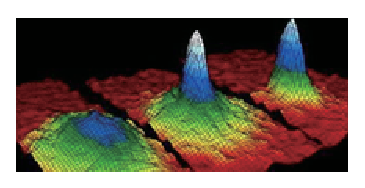
\includegraphics[width=0.7\textwidth]{figures/chap01/1-1BEC.eps}
\vspace{-10pt}
\caption{\label{fig.1-1}玻色―爱因斯坦凝聚。铷原子气的BEC(左图为BEC出现前;中图为BEC刚出现;右图为进一步蒸发后遗留的近乎纯净的BEC)\cite{Guo2016},图源自文献\cite{Guo2016}。}
\end{figure}










 
